\documentclass[12pt, letterpaper]{article}
\usepackage[spanish]{babel} % Carga el paquete para el idioma español
\usepackage[T1]{fontenc}    % Codificación de la fuente
\usepackage[utf8]{inputenc} % Codificación de entrada para caracteres UTF-8
\usepackage{graphicx} %LaTeX package to import graphics
\title{TEMAS DE HEURISTICA}
\author{Polya}
\date{2024 - Septiembre}
\begin{document}
\maketitle
Este artículo presenta los resultados de la
investigación cuyo propósito fue evaluar
la \emph{eficacia} del método heurístico de \textbf{\textit{Polya}}
\begin{figure}[ht] % 'ht' para que la figura esté aquí o en la parte superior
    \centering % Centra la imagen
    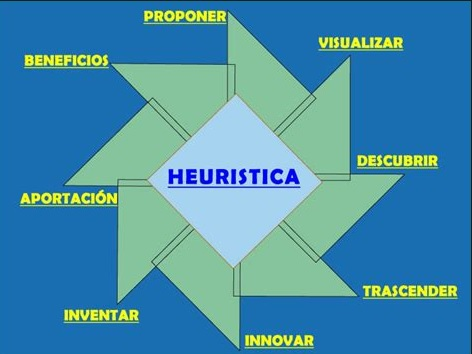
\includegraphics[width=0.8\textwidth]{heuristica.jpg} % Ajusta el ancho al 80% del texto
    \caption{Descripción de la imagen heurística.} % Pie de figura
    \label{fig:heuristica} % Etiqueta para referencias cruzadas
\end{figure}
\end{document}